\chapter{Objectifs, définitions, contraintes}
\section{Introduction aux réseaux wifi}

Le wifi, abréviation de wireless fidelity, est un ensemble de protocoles permettant la communication sans fil entre deux
appareils en utilisant des ondes radios. Ces protocoles se situent au niveau de la couche d'accés du modèle tcp/ip.
La standardisation de cette norme a été initiée l'IEEE\footnote{Institute of Electrical and Electronics Engineers} en 1990.
Cela a aboutit, en 1997, au standart IEEE 802.11 définissant les réseaux locaux sans fils \cite{WFintro}.
La norme d'origine prévoyait l'utilisation d'ondes radios dans la bande de fréquences libre entre 2401 et 2495 MHz,
couramment appelée bande à 2,4 GHz, ou d'infra rouges. Cependant, pour suivre l'évolution des technologies, le standart IEEE 
802.11 s'est enrichi afin d'augmenter le débit et d'utiliser la bande de fréqences libre entre 5170 et 5710 MHz.
Les standarts IEEE 802.11a et IEEE 802.11b ont donc été définis en 1999, le standart 802.11g et 2003 et le standart 802.11n
en 2009.

Depuis sa création, la norme IEEE 802.11 définit 14 canaux dans la bande 2,4 GHz. Chaque canal à une largeur de 22 MHz et 
l'écart entre les centres de deux canaux successifs est de 5 MHz\footnote{Sauf les centres des cannaux 13 et 14 qui sont espacés
de 12 MHz}. Il en résulte donc un fort recouvrement entre les différents canaux comme le montre la figure 1.1.

\begin{figure}
   \centering
   
\includegraphics[width=0.8\textwidth,natwidth=610,natheight=642]{images/cannaux.png}
   \caption{Répartition des canaux dans la bande 2,4 GHz}
\end{figure}

Un réseau wifi est un réseau local découpé en ``cellules'' appelées BSS\footnote{Basic Service Set}. Deux appareils
doivent se trouver dans le même BSS pour communiquer entre eux. Il existe deux modes de BSS : Le mode Infrastructure et le
mode ad-hoc\cite{WFfunc2}. La plupart des réseaux wifi de particuliers ou d'entreprises sont des réseaux en mode Infrastructure.

Le mode infrastructure est une topologie centralisée. Il se caractérise par le fait que chaque BSS posséde une station de
base, appelée aussi point d'accés, et que toutes les communications passent nécessairement par le point d'accés de la BSS,
et ce même si l'émetteur et le récepteur du message se trouvent dans le même BSS. Un point d'accés peut être relié par un réseau
cablé à un ou plusieurs autres points d'accés, étendant ainsi le LAN\footnote{Local Area Network, ou Réseau local}
\cite{WFfunc},ou à un routeur pour accéder à un réseau WAN\footnote{Wide Area Network, ou Réseau étendu}.
Le mode ad-hoc, au contraire, est un mode ``d'égal à égal''. Deux entités au sein du même BSS peuvent communiquer directement.


Comme le montre la figure 1.2\cite{WFhead}, le premier champ de l'en-tête wifi est le FCF\footnote{Frame Control Field, ou Champ
de contrôle de trame}, permettant d'identifier les trames en fonction de leur rôle. Ainsi, les trames peuvent être de trois types,
identifiées par les deux bits en position 3 et 4 du FCF : Management, Contrôle ou Donnée.\cite{WFfcf}. Les 4 bits suivants
identifient le sous type, et les 8 derniers bits sont des flags. Les trames de données sont utilisées pour transporter des données
de plus haut niveau, les trames de contrôles sont utilisées pour les acquittements et les réservations, et les trames de management
servent à organiser et maintenir le réseau\cite{MNfunc}.

Les Beacons frames sont des trames de management particulières qui permettent à un point d'accés de déclarer sa présence aux
appareils à proximité. Ils transportent différentes informations comme le SSID\footnote{Service Set IDentifier} du réseau,
qui est une chaîne de 2 à 32 caractères, un timestamp permettant de se synchroniser, le canal sur lequel il émet, 
et d'autres informations.\cite{WFfunc2}.
\begin{figure}
   \centering
   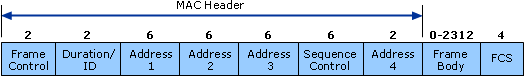
\includegraphics[width=0.8\textwidth,natwidth=488,natheight=513]{images/header_wifi.png}
   \caption{Format des trames 802.11}
\end{figure}

\section{La norme 802.11s}
Comme dit précédemment, le mode infrastructure est actuellement le plus utilisé. Cependant, une de ces limites est
que, dans certaines situations, il n'est pas toujours possible de connecter un point d'accés à un switch\cite{MNintro}.
En effet, la longueur des cables ethernet est limitée, ce qui rend difficile le déploiement de points d'accés dans des
environnements ouverts.

C'est ce qui fait la force du mode ad-hoc. Chaque appareil peut communiquer avec tous les autres appareils qui sont à portée.
De plus, chaque appareil peut relayer le message si le destinataire final n'est pas à portée. Ainsi, dans l'exemple de
la figure 1.3, chaque noeud peut communiquer avec nimporte quel autre, à la condition qu'un alogrithme de routage s'exécute
sur le réseau et que chaque noeud sache quel est le suivant pour atteindre la destination. Ce genre de réseau est appelé réseau
maillé\footnote{Mesh Network en anglais}. Le principal avantage de ces réseaux est qu'ils sont trés flexibles. On peut les étendre
sans avoir à tirer de nouveaux cables ou à ajouter de nouveaux équipements intermédiaires\cite{MNintro}. De plus, le retrait d'un
petit nombre de noeuds ne doit pas empêcher le réseau de fonctionner s'il est possible de trouver des routes alternatives pour
les trames.
\begin{figure}
   \centering
   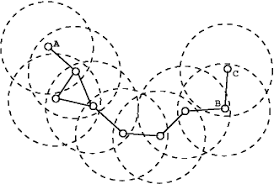
\includegraphics[width=0.8\textwidth,natwidth=488,natheight=513]{images/ad_hoc.png}
   \caption{Exemple de réseau ad-hoc}
\end{figure}

Le standart 802.11s est un amendement de la norme 802.11, définissant la manière dont les appareils disposant d'une carte réseau
sans fils peuvent s'interconnecter pour former un réseau sans fil maillé. L'IEEE a commencé à travailler sur ce standart en 
2003 et celui-ci a été adopté en 2006. Pour faciliter l'interopérabilité, un réseau 802.11s est vu de l'extérieur comme un
unique segment ethernet. Pour permettre la retransmission des informations d'un noeud à l'autre, la norme 802.11s
étend l'en-tête 802.11 classique avec un en-tête mesh comme montré dans la figure 1.4\cite{MNfunc}.

Les 4 champs d'adresses de l'en-tête 802.11 sont utilisés, puisqu'il faut à chaque transmission du message donner l'adresse
du noeud qui a effectué la transmission, celle du prochain noeud, celle du destinataire final et celle de l'expéditeur originel. 
Dans certains cas plus complexes, il est nécessaire d'ajouter des adresses supplémentaires, ce qui explique que l'en-tête mesh
comporte un champ optionel d'extention d'adresses. C'est le cas par exemple si l'émetteur et/ou le destinataire, ne se trouvent pas
dans le réseau mesh, mais que la trame va traverser un réseau mesh. Parmi les autres valeurs ajoutées, le TTL\footnote{Nombre de
fois maximal que peut être relayée une trame avant d'être abandonnée, cette valeur est décrémentée à chaque saut} et le Mesh sequence
number\footnote{nombre identifiant de manière unique une trame} permettent d'éviter les boucles infinies qui risqueraient de saturer
le réseau.


\begin{figure}
   \centering
   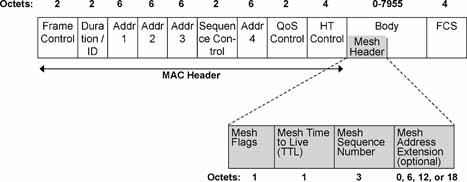
\includegraphics[width=0.8\textwidth,natwidth=488,natheight=513]{images/mesh_header.jpeg}
   \caption{Format des trames 802.11s}
\end{figure}

\section{Adressage et routage}

Dans un réseau TCP/IP, chaque noeud doit disposer de deux adresses. Chacune d'elles permet de l'identifier, en théorie, de manière 
unique. La première est l'adresse MAC, une adresse sur 48 bits, utilisée pour identifier les noeuds dans les protocoles de la 
couche d'accès du modèle TCP/IP. Cette adresse permet à une trame de voyager sur un LAN jusqu'à sa destination, mais sera changée
à chaque fois que le paquet passe par un routeur. La deuxième est l'adresse IP, une adresse sur 32 bits qui est utlisée par le
protocole IP, qui est un protocole de la couche réseau du modèle TCP/IP. Cette adresse est inchangée d'un bout de la transmission
à l'autre\footnote{en l'absence de mécanismes de traduction d'adresse (NAT)}.

L'adresse MAC est atribuée à une carte réseau par le constructeur. Ainsi, nous avons la garantie que chaque appareil possède une
adresse MAC unique. L'adresse IP doit également être unique mais, contrairement à l'adresse MAC, elle n'est pas enregistrée dans
la carte réseau par le constructeur car toutes les adresses IP identifiant les appareils d'un même LAN doivent avoir le même 
préfixe. Il existe des protocoles permettant d'affecter automatiquement des adresses IP à des appareils sans avoir besoin de
recourir à une intervention humaine. Le protocole majoritairement utilisé est DHCP\footnote{Dynamic Host Configuration 
Protocol}. Ce protocole nécessite qu'un serveur dispose d'une liste d'adresses IP disponibles qu'il va affecter à chaque noeuds
du réseau sur demande de ces derniers\cite{DHCP}. Néanmoins, le recours à un serveur central d'adresses IP amoindrit les 
avantages à l'utilisation d'une infrastructure décentralisée tel qu'un un réseau maillé.

Dans un réseau maillé, il est aussi nécessaire de prévoire le routage des trames. La norme 802.11s définit également le protocole
HWMP\footnote{Hybrid Wireless Mesh Protocol} comme protocole de routage pour les réseaux wifi maillés. Contrairement à la majorité 
des protocoles de routages, HWMP ne se base pas sur les adresses IP, mais sur les adresses MAC, puisque le but est d'aiguiller
les trames au sein d'un même LAN. Il s'agit d'un protocole de routage à vecteur distance puisque les noeuds n'ont pas conaissance
de l'intégralité de la topologie du réseau mais uniquement des noeuds qui le constituent et de la ``distance'' de chacun d'eux
\cite{MNroute}.
